\section{Further Work}
The system that was produced adhered to all of the functional requirements that the client laid out at the beginning of the project, but that does not mean that all potential functionality has been implemented, or even that the system is truly complete. In this section some key areas of functionality have been identified and expanded upon, and provide a starting point for the maintainers of the software to focus on.\ \\
\ \\
The first of these areas is the routing system, specifically how the route between two points is calculated. Currently, the user is the main factor influencing how scenic a route is. It is expected they will select several key picturesque locations, and the drive between them will also be pleasant. However, this will not always be the case, and a good route could be spoiled with the transitions between two points, especially if the distance between the points is large. The reason for this is that the routing system provides the shortest path between any two selected points, rather than the most visually appealing. In future iterations of the project, it would be beneficial if some data mining was performed alongside the routing system, so that multiple routes could be generated, their pleasantness evaluated, allowing the system to pick the best looking journey. This would improve the quality of all the routes in the system, as well as further helping to achieve the main goal of the application: to improve the user's driving experience.\ \\
\begin{figure}[!ht]
	\vspace{-3mm}
	\begin{center}
		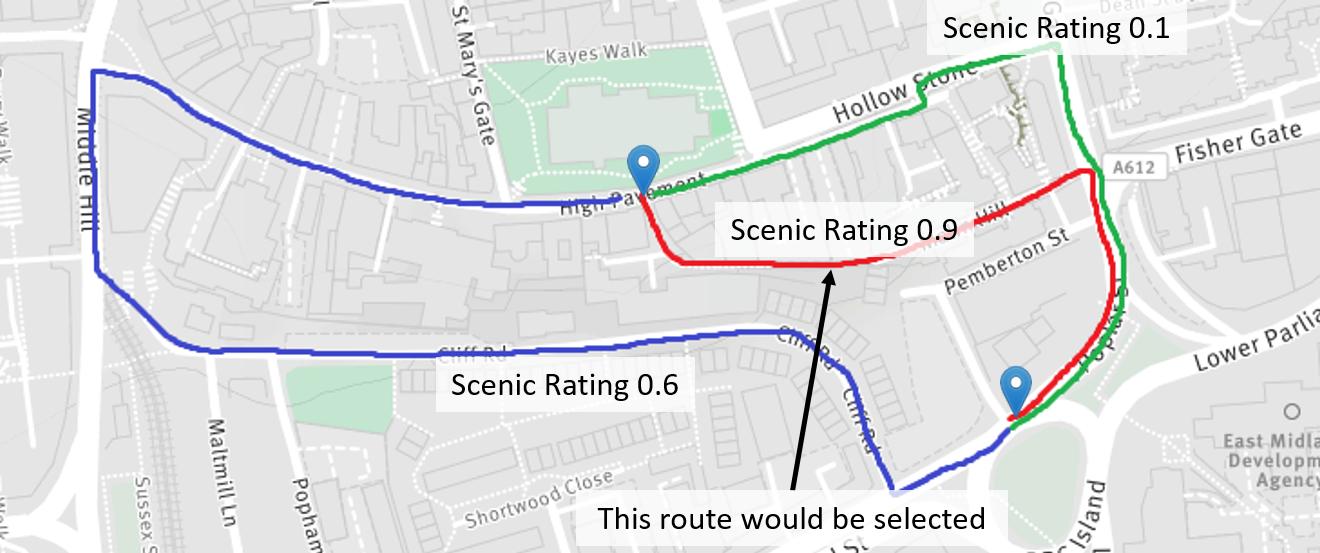
\includegraphics[width=0.9\textwidth]{images/further/alt.png}
	\end{center}
	\vspace{-6mm}
	\caption{Route recommendation based on some scenic rating}	
\end{figure}

\noindent 
Whilst on the topic of the route creation page, there are also other aspects which could be improved upon, by modifying the user interface, and adding more functionality. The first of these would be increasing the number of interactions possible, including the ability to change the order of points in the route, or the ability to add points in between other points. This would allow users to fix mistakes more easily, instead of having to delete segments of their route and reconstruct them. 
\ \\
\ \\
The other change to the route creation process would be to increase the diversity of routes, by allowing the addition of walking and cycling segments. This would allow users to add more to their routes, increase their quality, and improve how scenic they were. This would also be useful for expanding the user base to users that don't necessarily have cars, but still wish to experience peer recommended scenic routes.

\newpage 
\noindent 
The next area of future expansion would be the social interaction system. As it stands, the system provides support for users to have six interactions with routes: commenting, rating, sharing, downloading, cloning, and recommending similar routes. This is fine for users that don't use the site frequently, or don't visit a lot of routes, but for dedicated and recurrent users, it quickly becomes apparent there are some issues with managing their social interactions. There is no one central place where a user can view all the interactions that other users have had with them. This means that if a user wants to keep a track of this, they have to consistently check their emails, or visit each of their routes individually, which becomes much more difficult the more routes and interactions the user has. The solution to this problem is to implement some form of notification centre, where a user can see all the notifications they have received, similar in functionality to the notification system employed by Facebook. This would allow for users to review all of their notifications in a centralised place, so that they do not miss any, and do not need to check multiple locations for their notifications (which would not scale well as the number of sources of notifications, their routes, increases). This could then be further expanded with the ability to follow routes and other users of the system, so that notifications could be received for these as well.

\begin{figure}[!ht]
	\begin{center}
		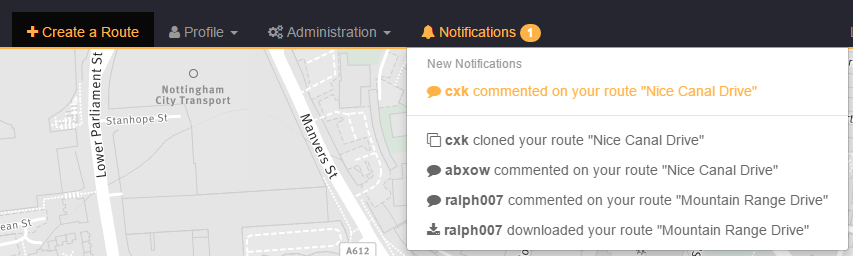
\includegraphics[width=0.9125\textwidth]{images/further/notification.png}
	\end{center}
	\vspace{-6mm}
	\caption{Mock up of the notification system, displaying all social interactions received}	
\end{figure}

\noindent 
The final area of further work is also an improvement on social interactions within the site, specifically the implementation of a site wide messaging system. This would allow for users to interact with one another on a much more personal level than simply commenting on each others routes. This deeper social interact could become one of the main driving features for users to returning to the site. It provides the ability for users to talk to users that provide quality content, friendships to form, and for groups with similar interests to develop. It would also mean that communication between members would be contained within the Niceway.to ecosystem, rather than users communicating on other social platforms, and potentially missing out on what's happening with their friends on Niceway.to. This freedom to communicate with other users would open up a lot of potential for Niceway.to and would increase the chance of users returning to the site on a regular basis (to check for any new messages).

\begin{figure}[!ht]
	\begin{center}
		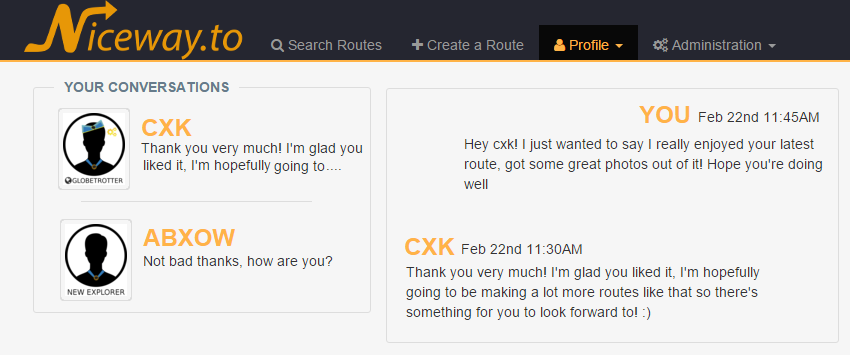
\includegraphics[width=0.85\textwidth]{images/further/chat.png}
	\end{center}
	\vspace{-6mm}
	\caption{Mock up of the chat system}	
	\vspace{-10mm}
\end{figure}

